\documentclass[12pt,twoside]{article}

%%%%%%% Loading packages and macros %%%%%%%
\usepackage{preamble/__packages__}
\usepackage{preamble/__macro__}
%%%%%%%%%%%%%%%%%%%%%%%%%%%%%%%%%%%%%%%%%%%

%%%%%%% Document %%%%%%%
\newcommand{\assignment}{ Assignment 3 }
\newcommand{\course}{FINC 585-3: Asset Pricing}
\newcommand{\prof}{Torben Andersen}
\newcommand{\institute}{Kellogg School of Management}

\title{\course-\assignment}
\author{TA: Jose Antunes-Neto}
\date{April 20, 2023}
%%%%%%%%%%%%%%%%%%%%%%%%

\begin{document}

\nocite{*}
\maketitle

\section{Problem 1.}
The question is motivated by the original work of \citeauthor{hansen1982generalized}, contrasting the assumptions and empirical evidence for consumption-based asset pricing obtained via GMM versus maximum likelihood. I have posted quarterly data in a file labeled HS.xlsx, containing time series on U.S. aggregate real private consumption and real value of the S\&P500 index covering 1958:Q1 to 2016:Q4.

Consider a representative agent who maximizes utility,
\[
    \sum_{t=0}^\infty \beta^t u(C_t)
\]
subject to the budget constraint:
\[
    W_{t+1}=(W_t-C_t) \cdot R_{t+1}^m
\]
where \(C_t\) is real consumption, \(W_t\) is real wealth, \(R_{t+1}^m\) is the gross real return on the market portfolio, which is a weighted sum of individual asset returns. That is, \(R_{t+1}^m = \sum_i \alpha^iR_{t+1}^i\), \(\alpha^i\) is the weight of asset \(i\) in the market portfolio , and \(R_{t+1}^i\) is gross real return on asset \(i\).

Optimization on the part of the agent implies that,
\[
    u^\prime(C_t) = \mathbb{E}_t\left[\beta R_{t+1}^m u^\prime(C_{t+1})\right]
\]
The left hand side of the above Euler equation is the increased utility from consuming one more unit of goods today. The right hand side is equal to the expectation of the present value of the increased utility, if the consumer invests one unit in the market portfolio today and consumes the gross return tomorrow. In equilibrium, the equality holds.

Let the utility function be given in terms of power utility (CRRA),
\[
    u(C_t) = \frac{C_t^{1-\gamma}-1}{1-\gamma}    
\]
Then the above Euler equation becomes,
\[
    1 = \mathbb{E}_t\left[R^m_{t+1}\beta\left(\frac{C_{t+1}}{C_t}\right)^{-\gamma}\right]
\]
Rewrite the above equation, letting \(F_t\) denote all information available at time \(t\),
\begin{equation}
    \label{eq:eq1}
    \bexpvalue{R^m_{t+1}\beta\left(\frac{C_{t+1}}{C_t}\right)^{-\gamma}-1 \Bigg\vert F_t} = 0
\end{equation}
\begin{enumerate}[label = \Alph*)]
    \item First, we do something unusual, partially to display the versatility of GMM, but also to guide us towards good starting values for a traditional GMM procedure. Equation~\ref{eq:eq1} contains two parameters and translates into one (unconditional) moment condition. You will impose specific values on these parameters and check if the resulting moment condition is close to be satisfied – without estimating any parameters. Simply fix \(\beta = 0.99\) and, for a grid of likely \(\gamma\) values, compute the GMM criterion function. That is, for each value of \(\gamma\) , compute the J-criterion using an efficient GMM procedure. Estimate the spectral density for the moment condition at frequency zero (the long-run variance) using a Bartlett (Newey-West) kernel with a cut-off' parameter that is appropriate given the persistence in the data. Plot the value of the criterion function for the different values of \(\gamma\). Discuss the results.
    \begin{solution}
        The returns are shown in Figure~\ref{fig:series}:
        \begin{figure}
            \centering
            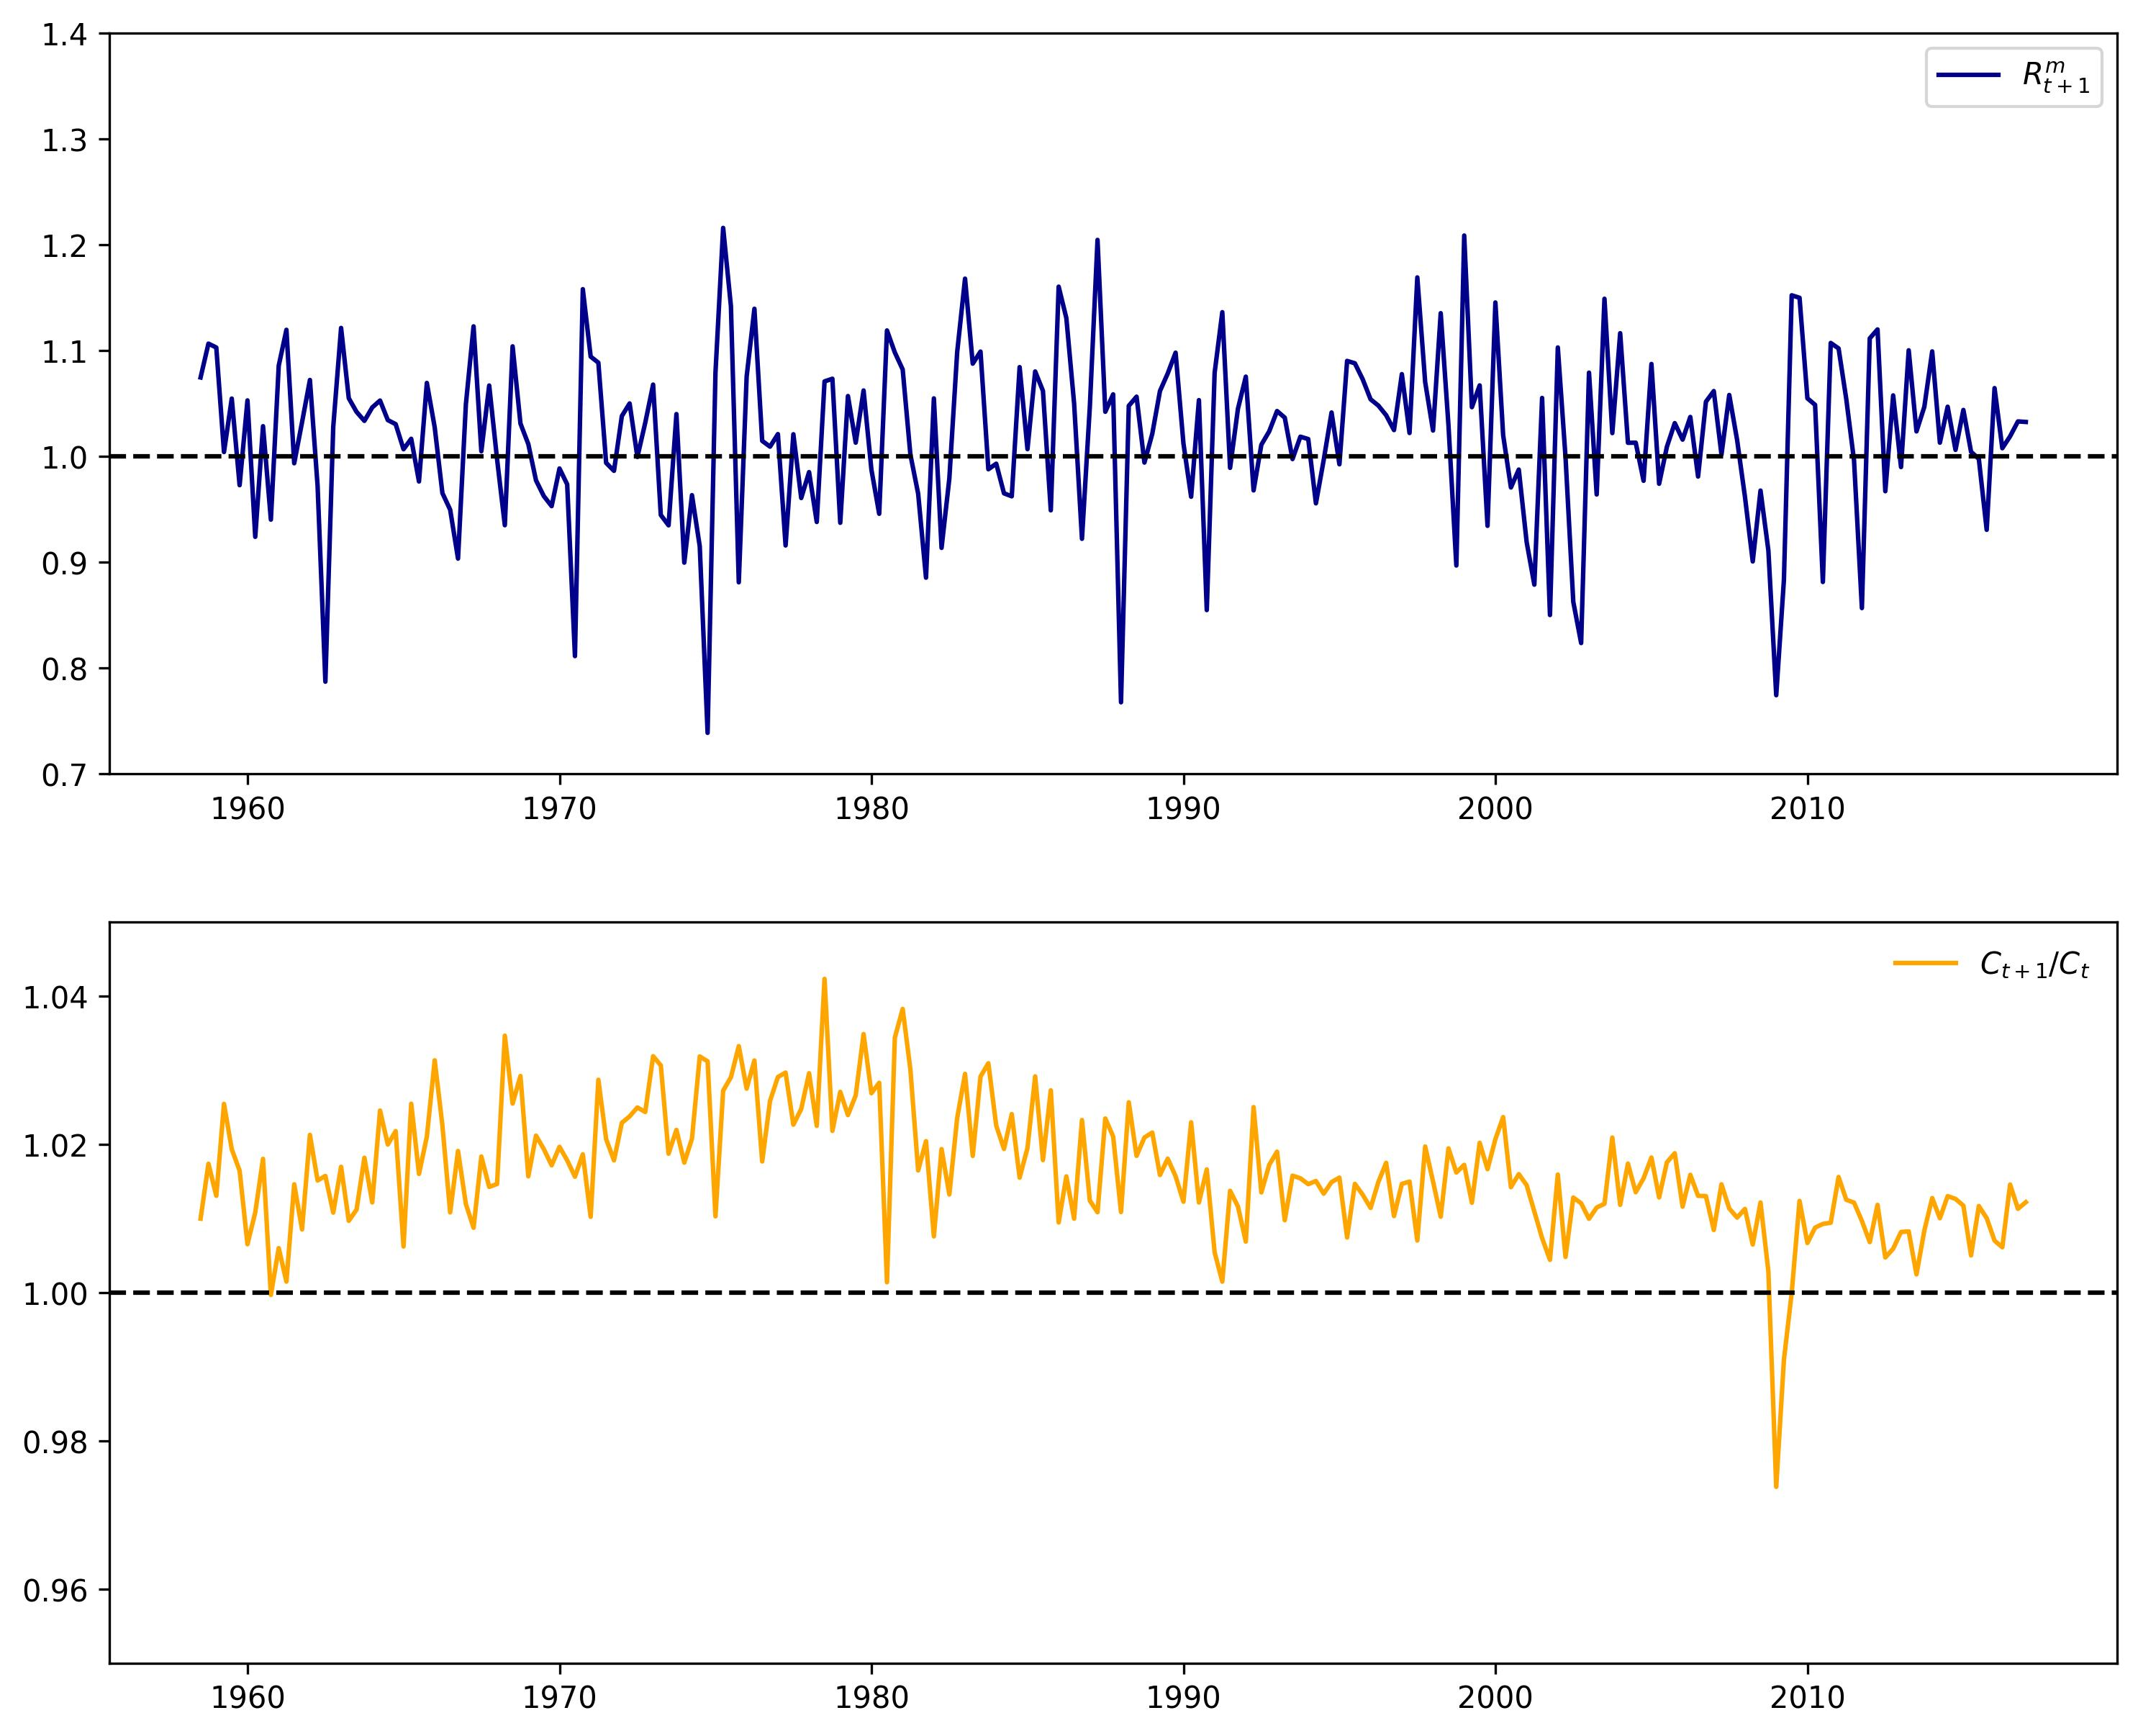
\includegraphics[width = .8\textwidth]{images/series.jpg}
            \caption{Series of \(R_t\) and \(C_t\) from 1958:Q1 to 2016:Q4}
            \label{fig:series}
        \end{figure}
        We start by defining some notation for this question. Following the lecture notes we denote 
        \[
            m(z_t, \theta) = m\left(\left(R_{t+1}^m, C_t, C_{t+1}\right), \left(\beta, \gamma\right)\right) = R^m_{t+1}\beta\left(\frac{C_{t+1}}{C_t}\right)^{-\gamma}-1
        \]
        and \(g_t(\theta) = T^{-1}\sum_t m(z_t, \theta)\) and \(\widehat S_T(\theta) =T^{-1}\sum_t m(z_t,\theta)^2\). Therefore the J-criterion of the GMM estimator is given by
        \[
            J_T(\theta) = g_T(\theta)^\prime \widehat S_T(\theta)^{-1} g_T(\theta)
        \]
        I then calculate the J-criterion for a grid of \(\gamma\) from 0 to 10 with length 1000. I used both the efficient weighting matrix (\(\widehat S_T\)) and the identity matrix. The results are shown in Figure~\ref{fig:jcrit} and the optimal value of gamma seems to be close to 1 for both criteria.
        \begin{figure}[!htbp]
            \centering
            \caption{J-criterion for the grid of \(\gamma\)}
            \label{fig:jcrit}
            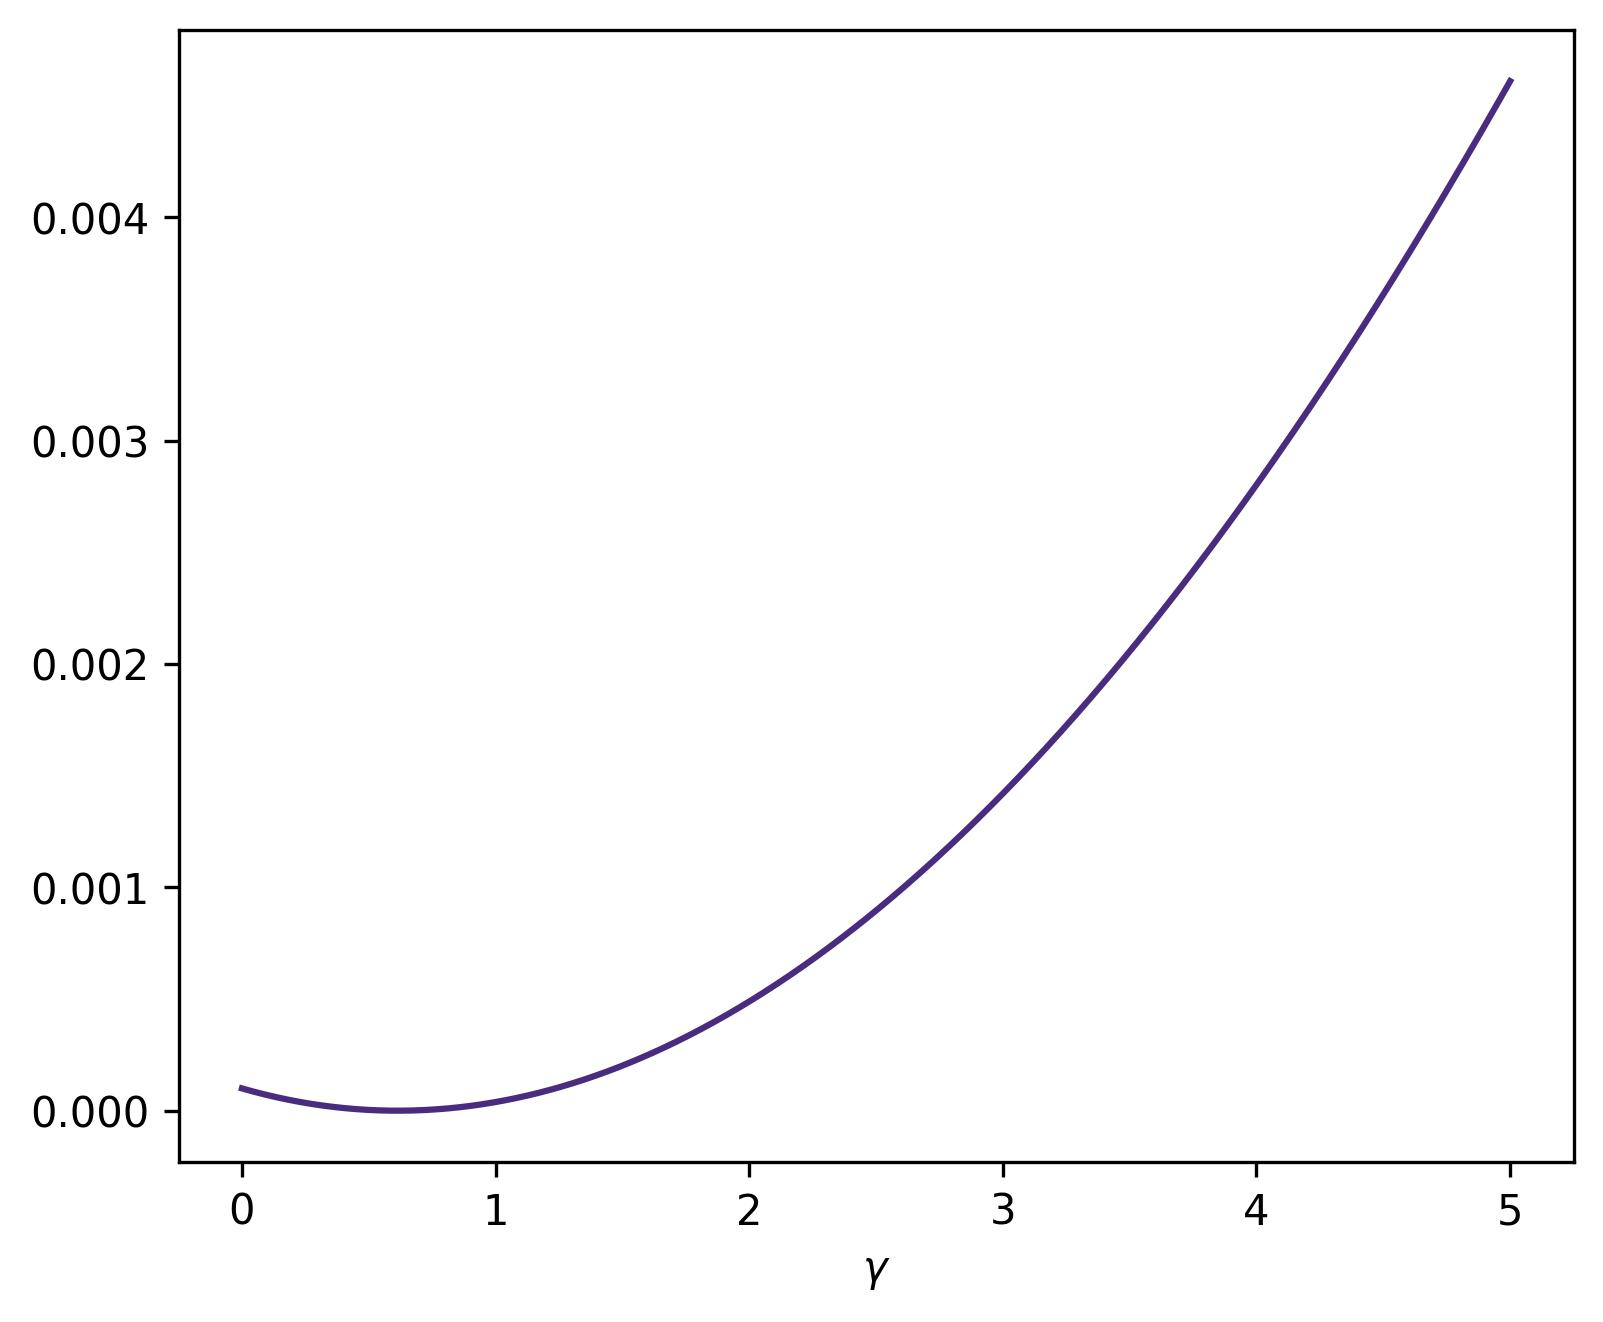
\includegraphics[width=0.6\textwidth]{images/jcrit.jpg}
        \end{figure}
    \end{solution}
    \item Repeat the procedure in question A), but letting \(F_t\) be represented by the instrument set: \(Z_t = \left(1, C_{t-1}, R^m_{t-1}\right)\), i.e., a constant and one-quarter lags of consumption growth \(C_{t-1}\)  and real returns. You are now exploiting over-identifying restrictions generated by the model.
    \begin{solution}
        Using the conditional moment from Equation~\ref{eq:eq1}, we can use the instruments \(Z_t\) to write
        \[
            \pexpvalue{m(z_t, \theta) Z_t} = 0
        \]
        so letting \(\tilde m(z_t, \theta, Z_t) = m(z_t, \theta) Z_t\) we can rewrite the J-criterion and the efficient matrix as
        \begin{align*}
            \tilde S_t(\theta) & = T^{-1} \sum_t \tilde m(z_t, \theta, Z_t) \tilde m(z_t, \theta, Z_t)^\prime = T^{-1} \sum_t m(z_t, \theta)^2 Z_t Z_T^\prime \\
            \tilde J_T(\theta) & = g_T(\theta)^\prime \tilde S_T(\theta)^{-1} g_T(\theta) 
        \end{align*}
        I then calculate this criteria as in the previous question and display it in Figure~\ref{fig:jcrit_cond}. The results remain the same.
        \begin{figure}[!htbp]
            \centering
            \caption{J-criterion for the grid of \(\gamma\) using the instruments \(Z_t\)}
            \label{fig:jcrit_cond}
            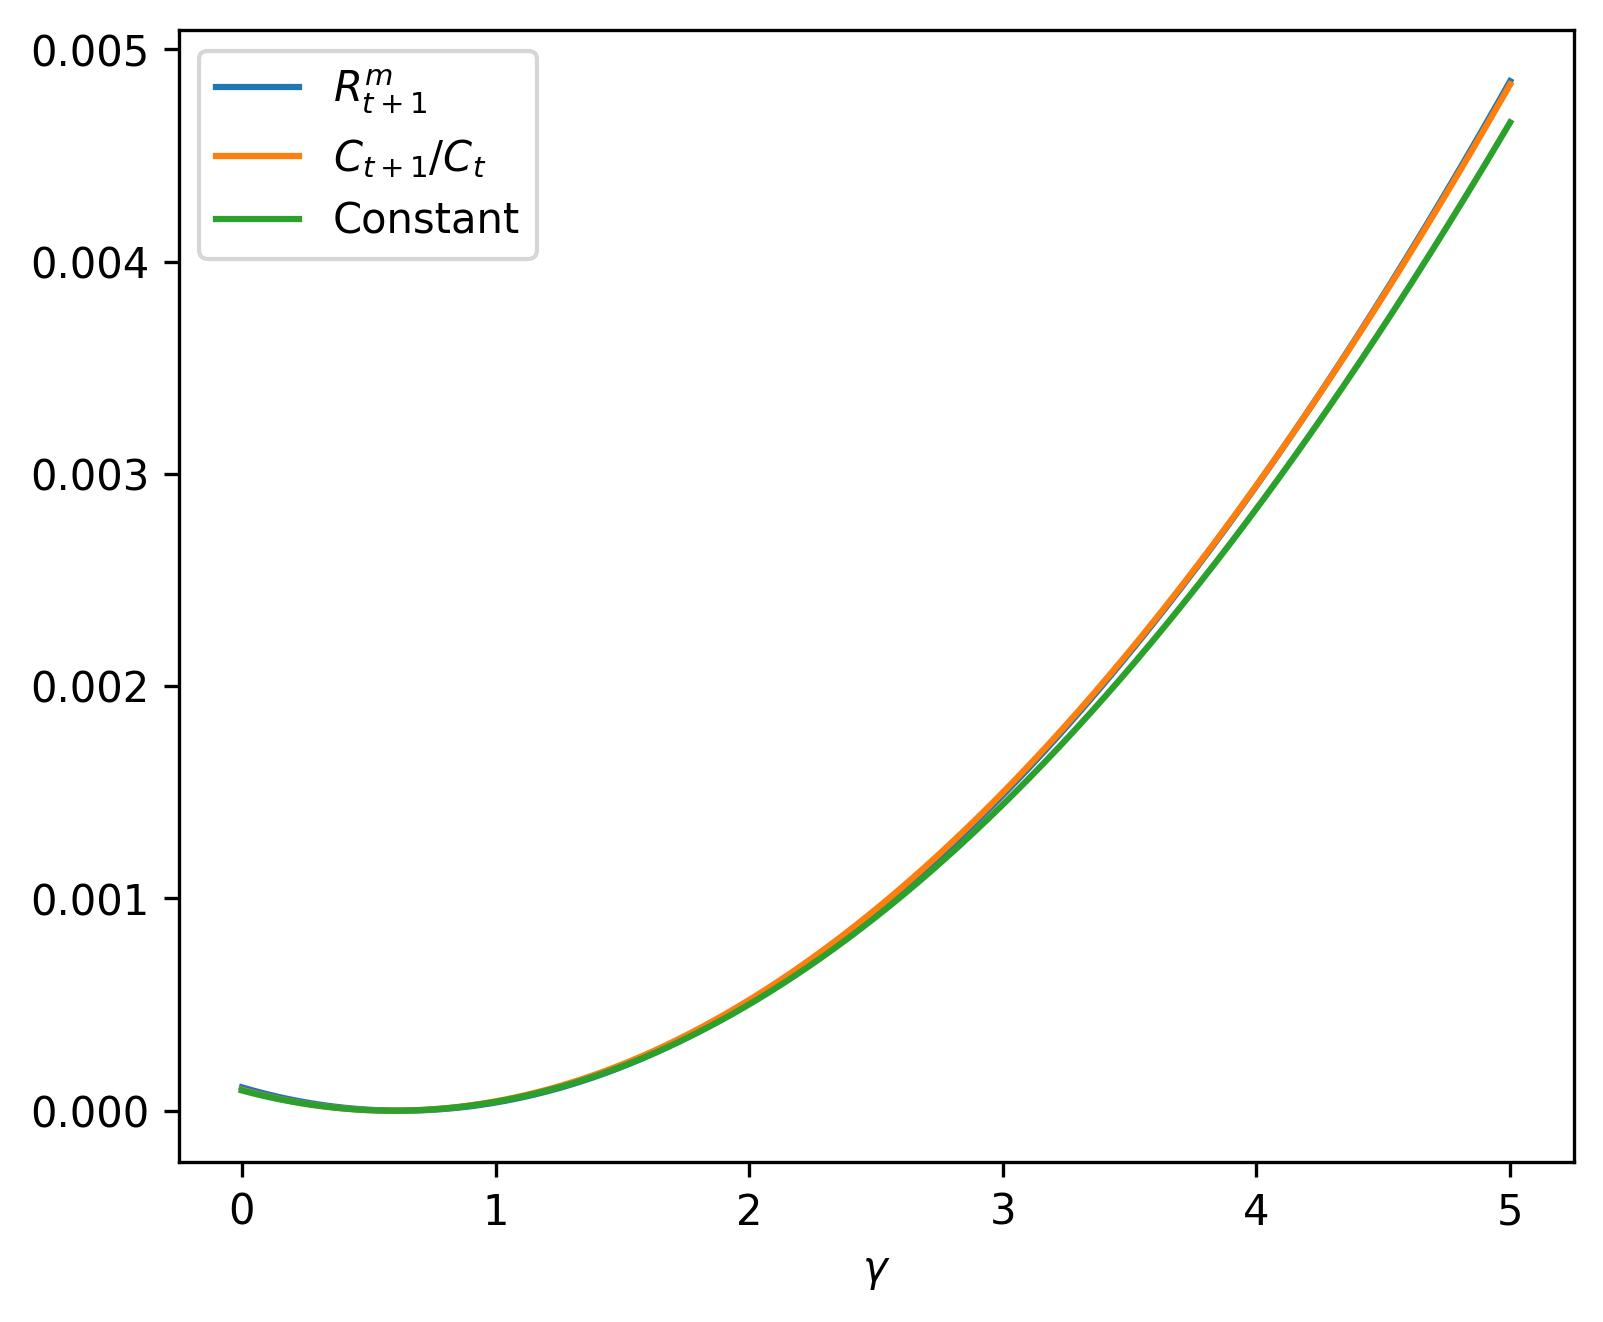
\includegraphics[width=0.6\textwidth]{images/jcrit_cond.jpg}
        \end{figure}
    \end{solution}
    \item Let us now try to perform actual parameter estimation with GMM. You have two free parameters, so you have to include moment conditions generated from (non-constant) instruments. Initially, estimate the system using the instruments in question B). You should now have a sense of reasonable values for the parameter vector, so you should have a good candidate for the original weighting matrix and do not have to estimate it using, say, the identity matrix. Report the parameter estimates, standard errors, and the J-test for the fit of the over-identifying restriction(s).
    \begin{solution}
        I estimate the parameters using a the first lag of \(R_t\) and \(C_t\) as instruments as well as a constant. The model is estimated using the minimization of the moment conditions. For the minimization algorithm, I used as initial guess the value of \(\gamma\) that minimized the J-criterion in (a) with \(\beta = 0.99\). Since these parameters are restricted (\(\gamma > 0, \beta \in (0,1)\)) I reparametrized the model to allow the algorithm to search over the entire real line which facilitates the minimization. Therefore the model is taken with
        \[
            \gamma = \frac{1}{1+\exp^{-\tilde\gamma}} \hspace{25pt} \beta = \tilde\beta^2
        \]
        Initially I tried to perform a two-step approach to estimate the parameters using the identity weighting matrix in the first step and using these estimates to calculate the efficient weighting matrix by calculating \(\widehat S(\beta,\gamma)\). This however did not turn out so well as the determinant of the estimated \(S\) was nearly zero, making the second-step estimate very volatile. I then kept the first stage as my final results which are reported below with the standard deviations in parenthesis:

        \begin{center}
            \begin{tabular}{ccccc}
$\beta$ = & 0.9900 & & $\gamma$ = & 0.6084 \\
& (0.0154) & & & (0.9286)
\end{tabular}
        \end{center}

        As we can see, the estimates of \(\gamma\) are close to the ones guessed on item (a) and \(\beta\) is really close to 0. We also note that the variance of \(\gamma\) is really high.

        To understand the stability of the estimates, I reestimate the model using a set of 10.000 random initial guesses and store the solutions for each one of them. The distribution of these solutions are shown in Figure~\ref{fig:solutions}. The results indicate that there may be two local solutions based on the modes of the marginal distribution in Figure~\ref{fig:solutions}. This presents a challenge to the estimation since it 

        \begin{figure}[!htbp]
            \centering
            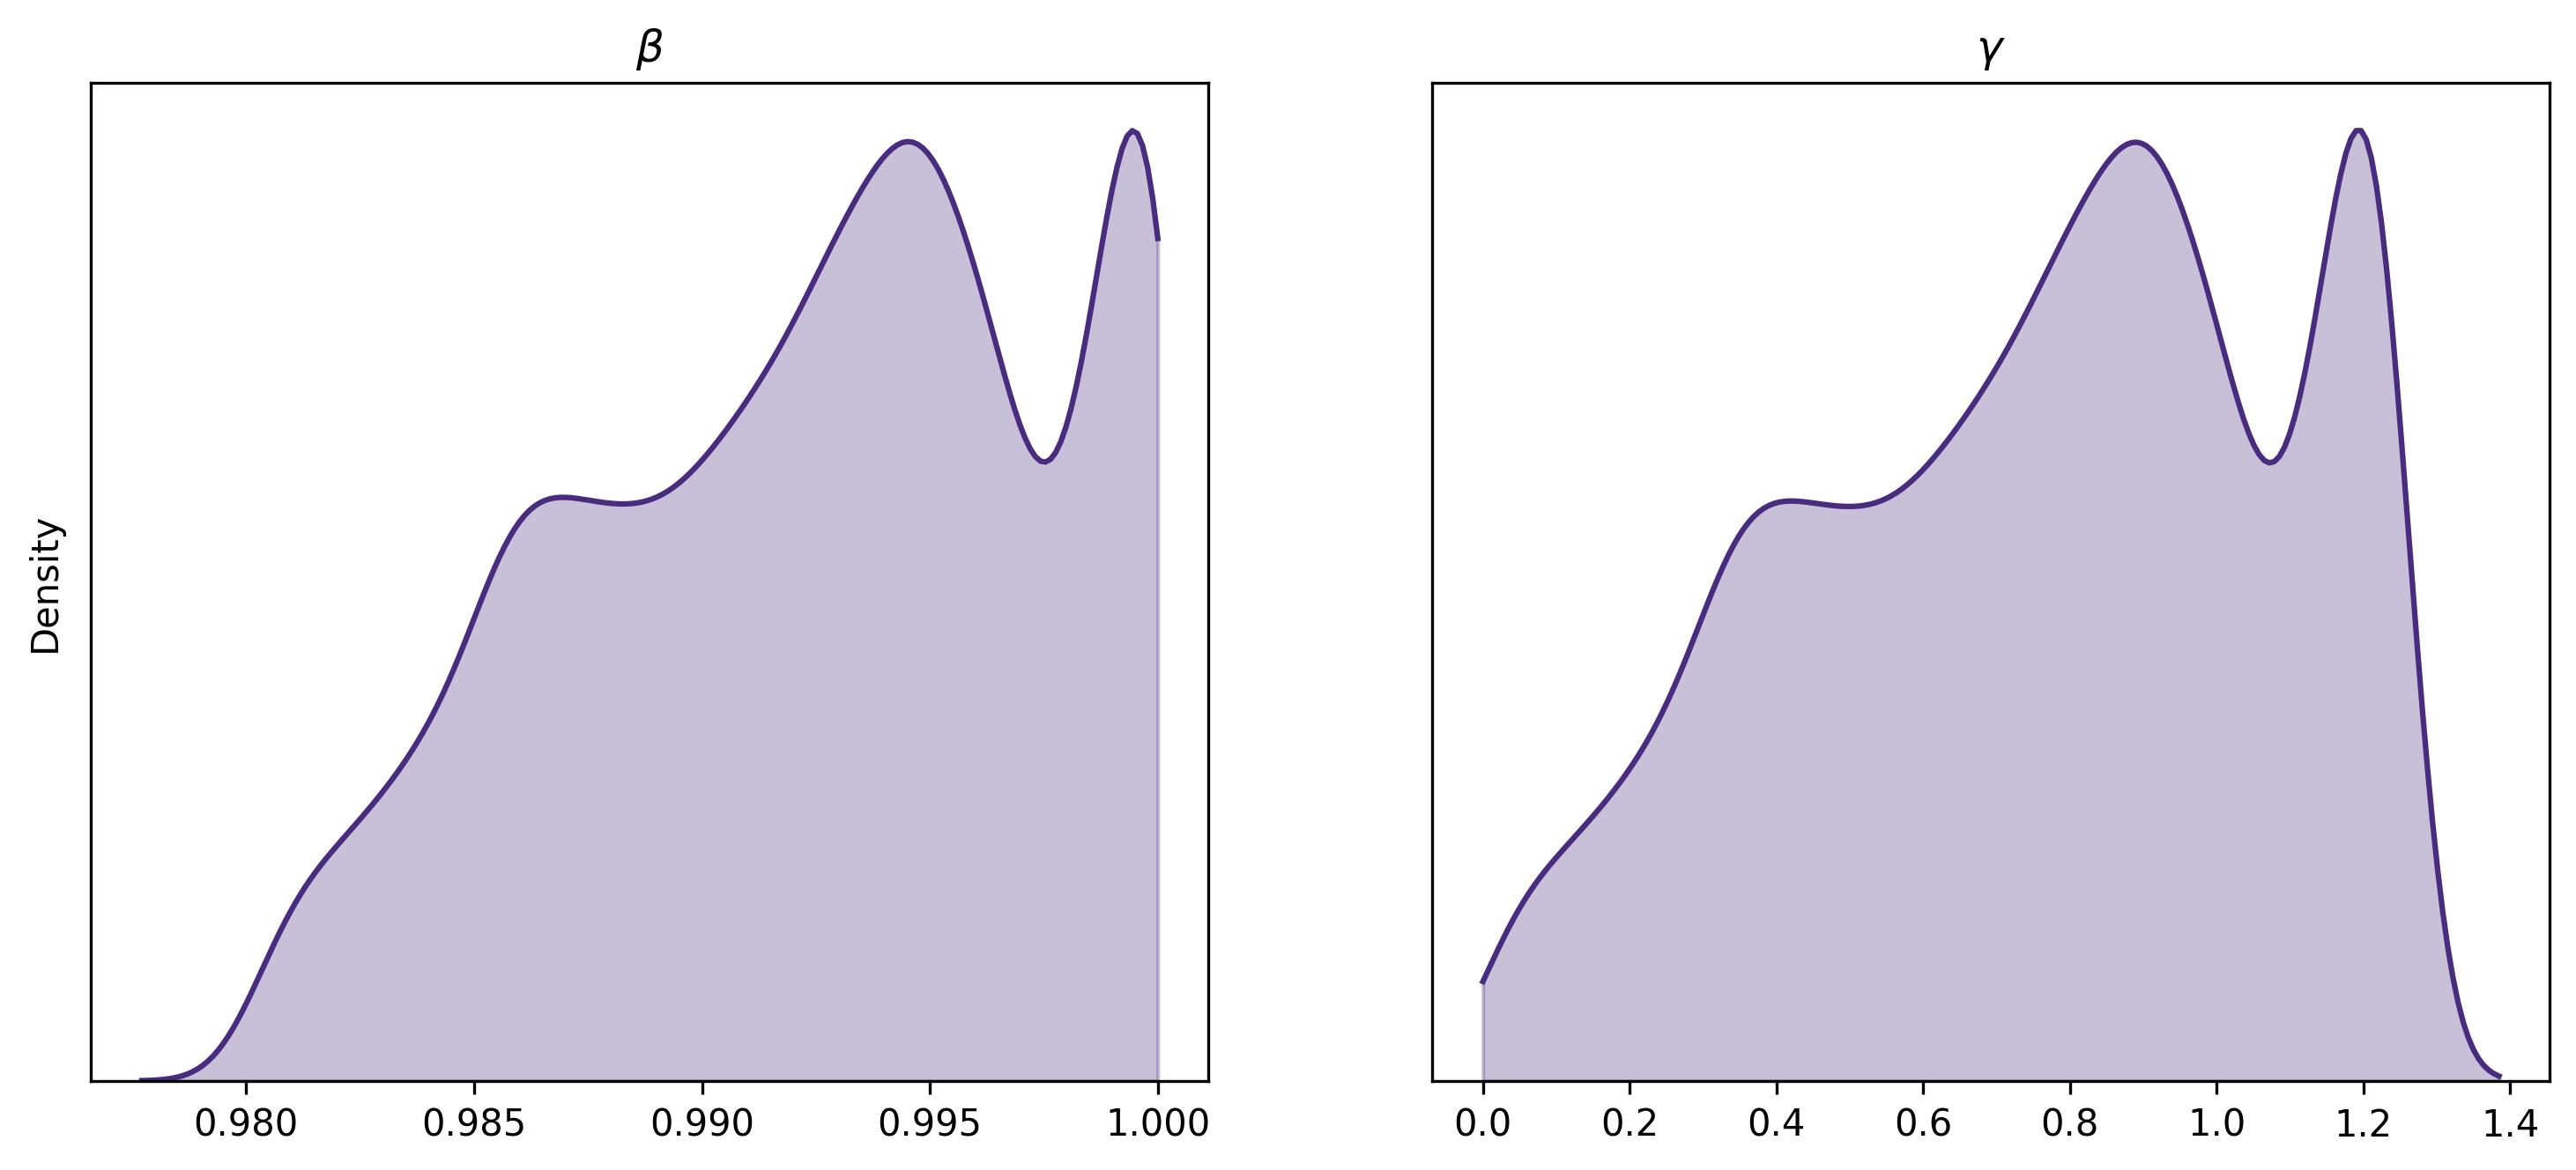
\includegraphics[width = \textwidth]{images/marg_solutions.jpg}
            \caption{Solutions for 10.000 random initial guesses}
            \label{fig:solutions}
        \end{figure}

        I now perform the Hausman test of overidentified restrictions whose null hypothesis is that a subset of the instruments is exogenous. If that is the case, then excluding (some) of the instruments would lead to a more efficient estimator. We analyze this by comparing the moment condition of both estimates. Under the null, a subset of the instruments can be used in a just-identified model to efficiently estimate the parameters. Under a just-identified model, the moment condition is perfectly matched and has zero average in the sample. Also, using the results of the previous problem set, we can compare an efficient and a consisent (but not efficient) estimator using the Hausman test. The test statistic is given by:
        \[
            \mathcal H = T \times \left[\frac{1}{T}\sum_{t=1}^T m\left(z_t, \widehat\theta\right)\right]^\prime A \left[\frac{1}{T}\sum_{t=1}^T m\left(z_t, \widehat\theta\right)\right]
        \]
        The results are shown below:
        \begin{center}
            \begin{tabular}{ccccc} 
$\chi^2$ =& 4.5339 & & p-value =& 0.9668 
\end{tabular}
        \end{center}
        As we can see, the test is not able to reject the null so there may be exogenous instruments.
    \end{solution}
    \item Expand the instrument set in question C) to include two, three, and four lags of the consumption growth and market return. For each set of (two) additional instruments, repeat the GMM estimation and report the results. In this case, you must obtain estimates for the weighting matrix in an initial step.
    \begin{solution}
        I calculate the model using 1, 2, 3 and 4 lags of the instruments. The  estimates are shown below:
        \begin{center}
            \begin{tabular}{@{\extracolsep{5pt}}lcccc} 
\\[-1.8ex]\hline 
\hline \\[-1.8ex] 
& \multicolumn{4}{c}{\textit{Number of Lags}} \\ 
& (1) & (2) & (3) & (4) \\ 
\hline \\[-1.8ex] 
$\beta$ & 0.990& 0.990& 0.990& 0.990\\ 
& (0.016)& (0.014)& (0.014)& (0.013)\\ 
$\gamma$ & 0.575& 0.566& 0.563& 0.563\\ 
& (0.941)& (0.835)& (0.846)& (0.806)\\ 
\hline \\[-1.8ex] 
N & 231 & 231 & 231 & 231\\ 
 $\mathcal H$ & 1.922 & 6.366 & 6.493 & 7.137\\ 
 p-value & 0.834 & 0.988 & 0.989 & 0.992 \\ 
\hline \hline \\[-1.8ex] 
\end{tabular}
        \end{center}
        The results are pretty similar all the set of instruments used and the interpretations of all the tests remain the same. We note that, as we increase the number of instruments, the estimation of \(\gamma\) gets more precise, judging by 
    \end{solution}
\end{enumerate}

\newpage 

\section{Problem 2.}
\citep{stambaugh1999predictive}. You will examine the bias in the slope coefficient in the regression of returns on past dividend yields, when the dividend yield process is highly persistent. Let \(y_t\) denote the return and \(x_t\) the dividend-price ratio (dividend yield) at date \(t\). Consider the following regression equations,

\begin{align*}
    y_t &= \alpha + \beta x_{t-1} + u_t \\
    x_t &= \theta + \rho x_{t-1} + v_t
\end{align*}

for \(t = 1, \dots, T\) and where,
\[
    \begin{bmatrix} u_t \\ v_t \end{bmatrix} \sim N(\mathbf 0_2, \Sigma)
\]

We can write the above equations in matrix form as follows,
\begin{align*}
    \mathbf{y} & = \alpha + \beta\mathbf{x} + \mathbf{u} \\ 
    \mathbf{x}^{+} & = \theta + \rho\mathbf{x} + \mathbf{v}
\end{align*}
where,
\begin{align*}
    \mathbf y & = \begin{bmatrix} y_1 & \cdots & y_T \end{bmatrix}^\prime \\
    \mathbf x & = \begin{bmatrix} x_0 & \cdots & x_{T-1} \end{bmatrix}^\prime \\
    \mathbf x^{+}  & = \begin{bmatrix} x_1 & \cdots & x_T \end{bmatrix}^\prime \\
    \mathbf u & = \begin{bmatrix} u_1 & \cdots & u_T \end{bmatrix}^\prime \\
    \mathbf v & = \begin{bmatrix} v_1 & \cdots & v_T \end{bmatrix}^\prime \\
\end{align*}

\begin{enumerate}[label = (\alph*)]
    \item  Show that 
    \[
        \widehat\beta = \beta + \begin{bmatrix}
            \mathbf{0} & \mathbf{1} 
        \end{bmatrix}(\mathbf{X}^\prime \mathbf{X})^{-1}\mathbf{X}^\prime \mathbf{u}
    \]
    where \(\mathbf{X} = \begin{bmatrix} \mathbf{1}_T & \mathbf x \end{bmatrix}\)
    \begin{solution}
        Since
        \[
            \mathbf y_t = \alpha + \beta \mathbf x + \mathbf u = \theta\mathbf X + \mathbf u
        \]
        Where \(\mathbf X = \begin{bmatrix} \mathbf 1_T & \mathbf x \end{bmatrix}\) and \(\theta = (\alpha , \beta)\). Then the usual OLS estimator of \(\theta\) is given by
        \[
            \widehat \theta = \left(\mathbf X^\prime \mathbf X \right)^{-1}\mathbf X^\prime \mathbf y
        \]
        Therefore \(\beta = \begin{bmatrix} 0 & 1 \end{bmatrix}\theta \) and
        \begin{align*}
            \widehat\beta & = \begin{bmatrix} 0 & 1 \end{bmatrix}\widehat\theta \\
            & = \begin{bmatrix} 0 & 1 \end{bmatrix}\left[\theta + \left(\mathbf X^\prime\mathbf X\right)^{-1}\mathbf X \mathbf u\right] \\
            & = \beta + \begin{bmatrix} 0 & 1 \end{bmatrix} \left(\mathbf X^\prime \mathbf X\right)^{-1}\mathbf X^\prime \mathbf u
        \end{align*}
    \end{solution}
    \item Show that \(\mathbf{u}\) can be decomposed as \(\mathbf{u} = \frac{\sigma_{uv}}{\sigma_v^2}\mathbf v + \mathbf e\) where \(e\) is uncorrelated with \(v\), and,
    \[
        \widehat \beta = \beta + \frac{\sigma_{uv}}{\sigma_v^2}\begin{bmatrix}
            \mathbf{0} & \mathbf{1}
        \end{bmatrix}\left(\mathbf{X}^\prime \mathbf{X}\right)^{-1}\mathbf{X}^\prime \mathbf{v} + \begin{bmatrix}
            \mathbf{0} & \mathbf{1}
        \end{bmatrix}\left(\mathbf{X}^\prime \mathbf{X}\right)^{-1}\mathbf{X}^\prime \mathbf{e}
    \]
    \begin{solution}
        Since \(u_t\) and \(v_t\) are jointly normal, then we can write that 
        \[
            u_t = \gamma v_t + e_t
        \]
        where \(e_t\) is uncorrelated with \(v_t\) and \(\gamma\) is given by the OLS coefficient \(\gamma = \frac{\sigma_{uv}}{\sigma_v^2}\) . Therefore we can rewrite the equation from the previous item as:
        \begin{align*}
            \widehat\beta & = \beta + \begin{bmatrix} 0 & 1 \end{bmatrix}\left(\mathbf X^\prime \mathbf X\right)^{-1}\mathbf X^\prime \mathbf u \\
            & = \beta + \begin{bmatrix} 0 & 1 \end{bmatrix}\left(\mathbf X^\prime \mathbf X\right)^{-1}\mathbf X^\prime  \left(\gamma \mathbf v + \mathbf e\right) \\
            & = \beta + \frac{\sigma_{uv}}{\sigma_v^2}\begin{bmatrix} 0 & 1 \end{bmatrix}\left(\mathbf X^\prime \mathbf X\right)^{-1} \mathbf X^\prime v + \begin{bmatrix} 0 & 1 \end{bmatrix}\left(\mathbf X^\prime \mathbf X\right)^{-1}\mathbf X^\prime \mathbf e
        \end{align*}
    \end{solution}
    \item Show that,
    \[
        \widehat \rho = \rho + \begin{bmatrix}
            \mathbf{0} & \mathbf{1}
        \end{bmatrix}\left(\mathbf{X} \mathbf{X}\right)^{-1}\mathbf{X} \mathbf{v}
    \]
    \begin{solution}
        Follows from the same logic as in the first item.
    \end{solution}
    \item Show that
    \[
        \bexpvalue{\widehat\beta-\beta} = \frac{\sigma_{uv}}{\sigma_v^2} \bexpvalue{\widehat\rho - \rho}
    \]
    and, using the expression \(\bexpvalue{\widehat\rho-\rho}\approx -\frac{1+3p}{T}\), for the finite sample bias of the estimated AR(1) coefficient from \citet{kendall1954note}, discuss the potential magnitude of the bias in \(\widehat\beta\) above, when \(T\) is 50 years, \(\rho = 0.94\) and \(\frac{\sigma_{uv}}{\sigma_v^2} = -1\).
    \begin{solution}
        Combining item (b) and (c) we can write that
        \begin{align*}
            \widehat\beta-\beta = \frac{\sigma_{uv}}{\sigma_v^2}\begin{bmatrix} 0 & 1\end{bmatrix}\left(\widehat\rho-\rho\right) + \begin{bmatrix}0 & 1 \end{bmatrix} \left(\mathbf X^\prime\mathbf X\right)^{-1}\mathbf X \mathbf e
        \end{align*}
        Then using the assumption that \(e_t\) is independent from \(\mathcal{F}_{t-1}\) (the information from the previous period, which contains the lagged \(\mathbf X\)), we can take the conditional expectation 
        \begin{align*}
            \mathbb E_{t-1}\left[\widehat\beta-\beta\right] & = \frac{\sigma_{uv}}{\sigma_v^2}\begin{bmatrix} 0 & 1\end{bmatrix}\mathbb E_{t-1}\left[\widehat\rho-\rho\right] + \begin{bmatrix}0 & 1 \end{bmatrix} \left(\mathbf X^\prime\mathbf X\right)^{-1}\mathbf X \mathbb E_{t-1}\left[\mathbf e\right] \\
            \mathbb E_{t-1}\left[\widehat\beta-\beta\right] & = \frac{\sigma_{uv}}{\sigma_v^2}\begin{bmatrix} 0 & 1\end{bmatrix}\mathbb E_{t-1}\left[\widehat\rho-\rho\right] \\
            \bexpvalue{\widehat\beta-\beta} & = \frac{\sigma_{uv}}{\sigma_v^2}\bexpvalue{\widehat\rho-\rho}
        \end{align*}
        Using the  expression from \citet{kendall1954note} that implies
        \[
            \bexpvalue{\widehat\beta-\beta}\approx -\frac{\sigma_{uv}}{\sigma_v^2}\frac{1+3p}{T}
        \]
        Using the proposed values of \(T = 50\), \(\rho = 0.94\) and \(\frac{\sigma_{uv}}{\sigma_v^2} = -1\) we would have a bias of \(\widehat\beta\) equal to \(0.0764\). Therefore, just from the persistence of the regressor, our estimator would be biased.
    \end{solution}
    \item Try to interpret the implications of your results for predictive regressions more generally. The issues highlighted here have generated a large literature!
    \begin{solution}
        This results suggest that the persistence of the regressors can be a real enemy when estimating a predictive regression. As we know, the more persistent the \(x\) (\(\rho \to 1\)) the harder it gets to estimate this parameter and the higher the estimation bias of the AR coefficients. This feeds back to the predictive equation by also increasing the bias of the estimated \(\beta\). This is a problem because we are interested in the predictive power of the regressor, but the more persistent it is, the harder it gets to estimate it and the more biased the estimated \(\beta\) will be. 
        The interpretation behind this is that, as \(x\) gets more persistent, shocks in the predictor tend to last longer, which makes it harder to estimate the real impact of \(x\) on \(y\).
    \end{solution}
    \item Design a small Monte Carlo study to explore the size of bias in finite samples by experimenting with different values for sample size, \(T\), the degree of persistence in the regressor, \(\rho\), and the (normalized) covariance between the innovations, \(\sigma_{uv}\) (or \(\sigma_{uv}/\sigma_v^2\)). Please report some relevant findings.
    \begin{solution}
        To start, I fix \(\beta = 1\) and \(\alpha = 0\). The errors \(u\) and \(v\) are set to have unit variance. Then I simulate the model varying the levels of \(T, \sigma_{uv}, \rho\):
        \begin{align*}
            T & \in \left\lbrace 50, 100, 150, \dots, 1000 \right\rbrace \\
            \sigma_{uv} & \in \left\lbrace -0.9, -0.8, \dots, 0.8, 0.9 \right\rbrace \\
            \rho & \in \left\lbrace 0, 0.3, 0.5, 0.9, 0.95, 0.99 \right\rbrace
        \end{align*}
        Every model is simulated 10.000 times and I calculate the average bias of \(\widehat\beta\) among these simulations. The results are shown in Figure~\ref{fig:bias} which displays the absolute level of the bias for each level of \(\rho\), \(\sigma_{uv}\) and \(T\). As we can see, the bias dies out quickly with T, but it is very sensitive to the level of persistence of the regressor. The higher the persistence, the higher the bias and the longer it takes to die out. The same happens with the covariance between the errors. The higher the covariance, the higher the bias and the longer it takes to die out. For higher levels of \(\rho\) such as 0.99, we see that the bias is still big for sample sizes around 150, which can sometimes be considered big.
        \begin{figure}[!htbp]
            \centering
            \includegraphics[width = \textwidth]{images/bias.jpg}
            \caption{Bias of the OLS estimator under different levels of \(\rho\), \(\sigma_{uv}\) and \(T\)}
            \label{fig:bias}
        \end{figure}
    \end{solution}
\end{enumerate}

\newpage

\section{Problem 3.}
This problem asks you to provide proofs of some results that wee cited in Lecture Notes 3.

\begin{enumerate}
    \item Provide proofs for all the results not proven on pages 4-5 of Lecture Notes
    \begin{solution}
        \setcounter{result}{1}
        \begin{result} 
            The Minimum Variance Portfolio, \textbf{MV}, is given by,
            \[
                \mathbf\omega_{MV} = \frac{\mathbf\Omega^{-1}\mathbf 1}{\mathbf 1^\prime\mathbf\Omega^{-1}\mathbf 1}
            \]
            with Mean and Variance,
            \[
                \frac{\mathbf{\mu}^\prime\mathbf{\Omega}^{-1}\mathbf{1}}{\mathbf{1}^\prime\mathbf{\Omega}^{-1}\mathbf{1}} = \frac{A}{C} \quad \text{and} \quad \frac{\mathbf{1}}{\mathbf{1}^\prime\mathbf{\Omega}^{-1}\mathbf{1}} = \frac{1}{C}
            \]
        \end{result}
        \begin{proof}
            The MV portfolio is characterized by the solution to the following problem:
            \[
                \mathbf\omega_{MV} \coloneqq \arg\min_{\mathbf\omega^\prime\mathbf 1 = 1} \mathbf\omega^\prime\mathbf\Omega\mathbf\omega
            \]
            Letting \(2\lambda\) be the lagrangian multiplier of the constraint we have the following first order condition:
            \[
                2\mathbf\Omega\mathbf\omega_{MV} - 2\lambda\mathbf 1 = 0 \iff \mathbf\Omega\mathbf\omega_{MV} = \lambda\mathbf 1 \iff \mathbf\omega_{MV} = \lambda\mathbf\Omega^{-1}\mathbf 1
            \]
            Using the binding constraint we can solve for \(\lambda\):
            \begin{align*}
                1 & = \mathbf\omega_{MV}\mathbf 1 \\ 
                1 & = \lambda \mathbf 1^\prime \mathbf \Omega^{-1} \mathbf 1 \\
                \lambda & = \frac{1}{\mathbf 1^\prime \mathbf \Omega^{-1} \mathbf 1} \eqqcolon \frac{1}{C}
            \end{align*}
            Substitutting back into the solution for \(\mathbf\omega_{MV}\) we have,
            \[
                \mathbf\omega_{MV} = \frac{\mathbf\Omega^{-1}\mathbf 1}{\mathbf 1^\prime \mathbf \Omega^{-1} \mathbf 1}
            \]
            The mean and variance of the MV portfolio are given by,
            \[
                \mathbf \mu^\prime \mathbf\omega_{MV}  = \frac{\mathbf\mu^\prime\mathbf\Omega^{-1}\mathbf 1}{\mathbf 1^\prime \mathbf \Omega^{-1} \mathbf 1} = \frac{A}{C} \quad \text{and} \quad \mathbf\omega_{MV}^\prime \mathbf \Omega \mathbf\omega_{MV} = \frac{\mathbf 1^\prime \mathbf \Omega^{-1} \mathbf 1}{\mathbf 1^\prime \mathbf \Omega^{-1} \mathbf 1} = \frac{1}{C}
            \]
        \end{proof}

        \begin{result}
            Associated with each Efficient Frontier Portfolio, \(\mathbf\omega_p\), there is a Unique (and Inefficient) Frontier Portfolio, \(\mathbf \omega_{pz}\), which is uncorrelated with the Former.
        \end{result}
        \begin{proof}
            For any MVF portfolio \(\mathbf\omega_p\) we can write,
            \[
                \mathbf\omega_p = \mathbf g + \mu_p\mathbf h
            \]
            where 
            \[
                \mathbf g^\prime \mathbf 1 = 1 \quad \mathbf g^\prime\mathbf\mu = 0 \quad \mathbf h^\prime\mathbf 1 = 1 \quad \mathbf h^\prime \mathbf \mu = 1
            \] 
            Using the previous result we can write \(\mathbf g\) and \(\mathbf h\) as functions of \(A,B,C\) and \(D \coloneqq BC-A^2\) as follows (you can verify that this is a solution to the system of equations above),
            \begin{align*}
                \mathbf g & = \frac{B}{D} \mathbf\Omega^{-1}\mathbf 1 - \frac{A}{D}\mathbf\Omega^{-1}\mathbf \mu \\
                \mathbf h& = \frac{C}{D} \mathbf\Omega^{-1}\mathbf \mu - \frac{A}{D}\mathbf\Omega^{-1}\mathbf 1
            \end{align*}
            Now fix 2 MVF portfolios \(p\) and \(pz\). They are uncorrelated iff
            \begin{align*}
                0 & = \mathbf\omega_p^\prime \mathbf\Omega \mathbf\omega_{pz} \\
                0 & =  \left(\mathbf g + \mu_p\mathbf h\right)^\prime \mathbf\Omega \left(\mathbf g + \mu_{pz}\mathbf h\right) \\
                0 & = \mathbf g^\prime \mathbf \Omega \mathbf g + \left(\mu_p+\mu_pz\right)\mathbf g^\prime\Omega\mathbf h + \mu_p\mu_{pq}\mathbf h^\prime\mathbf\Omega\mathbf h 
            \end{align*}
            Using the formulas for \(\mathbf g\) and \(\mathbf h\) this implies
            \begin{align*}
                0 & = \frac{B}{D} - \left(\mu_p+\mu_{pq}\right)\frac{A}{D} + \mu_p\mu_{pq}\frac{C}{D} \\
                \mu_{pq}\left(A - \mu_p C\right) & = B -\mu_pA \\
                \mu_{pq} & = \frac{B-\mu_pA}{A-\mu_pC}
            \end{align*}
        \end{proof}
    \end{solution}
    \item Provide the derivation for the optimal portfolio in the case where a risk-free asset is present on page 7 of Lecture Notes 3.
    \begin{solution}
        The optimal portfolio is defined as the soltuion to the following problem:
        \begin{align*}
            & \min_{\mathbf \omega} \mathbf\omega^\prime \mathbf\Omega \mathbf \omega \\
            & \text{s.t.} \quad \mathbf\omega^\prime \mu + \left(1-\mathbf\omega^\prime\mathbf 1\right)R_f = \mu_p \\
        \end{align*}
        Defining \(\mathbf{\tilde\mu} \coloneqq \mathbf \mu - R_f\mathbf 1\) as the respective excess returns we can rewrite the constraint as,
        \[
            \mathbf\omega\mathbf{\tilde\mu} = \tilde\mu_p
        \]
        Again using \(2\lambda\) as the lagrangian multiplier we can write the first order condition of the above problem as below
        \[
            \mathbf\Omega\mathbf\omega = \lambda \mathbf{\tilde\mu} \iff \mathbf \omega = \lambda \mathbf\Omega^{-1}\mathbf{\tilde\mu}
        \]
        Using the constraint:
        \[
            \tilde\mu_p = \mathbf\omega^\prime\mathbf{\tilde\mu} = \lambda\mathbf{\tilde\mu}^\prime\Omega^{-1}\mathbf{\tilde\mu} \iff \lambda = \frac{\tilde\mu_p}{\mathbf{\tilde\mu}^\prime\Omega^{-1}\mathbf{\tilde\mu}}
        \]
        so we conclude that
        \begin{align*}
            \mathbf\omega & = \tilde\mu_p \left(\mathbf{\tilde\mu}^\prime\mathbf\Omega^{-1}\mathbf{\tilde\mu}\right)^{-1}\mathbf\Omega^{-1}\mathbf{\tilde\mu} \\
            & = \underbrace{\frac{\tilde\mu_p\left(\mathbf 1^\prime\mathbf \Omega^{-1}\mathbf 1\right)}{\mathbf{\tilde\mu}^\prime\Omega^{-1}\mathbf{\tilde\mu}}}_{c_p} \underbrace{\frac{\mathbf\Omega^{-1}\mathbf{\tilde\mu}}{\mathbf 1^\prime \mathbf\Omega^{-1}\mathbf{\tilde\mu}}}_{w_q}
        \end{align*}
    \end{solution}
\end{enumerate}

$ $\clearpage
\bibliography{preamble/__references__}
\bibliographystyle{abbrvnat}

\end{document}